\documentclass[../TDM1-M2.tex]{subfiles}%

\begin{document}
\section[s]"2"{Étude d'un volant de badminton}

\enonce{%
	Un volant de badminton a une masse $m = \SI{5,0}{g}$. On veut vérifier
	expérimentalement l'information trouvée sur internet qui précise qu'un volant
	lâché de très haut atteint une vitesse limite $v_l = \SI{25}{km.h^{-1}}$. Pour
	tester cette affirmation, on veut déterminer l'altitude $h$ à laquelle il faut
	le lâcher (sans vitesse initiale) pour qu'il atteigne cette vitesse limite.
	\bigbreak
	On lâche le volant d'une fenêtre en hauteur et on filme sa chute verticale. On
	note O le point de départ de la chute, et (O$z$) l'axe vertical dirigé vers le
	bas. Au cours de la chute, on prend en compte une force de frottement due à
	l'air de la forme $\Ff = -\lambda v\vf$ où $\vf$ est le vecteur vitesse du point
	M, $v$ sa norme et $\lambda$ un coefficient positif. On note $g$ l'accélération
	de la pesanteur et on rappelle que $g = \SI{9,81}{m.s^{-2}}$.
}

\QR{%
	Établir l'équation différentielle portant sur la norme du vecteur
	vitesse $v(t)$.
}{%
	~
	\vspace{-15pt}
	\smallbreak
	\begin{itemize}
		\item[b]{Système}~: \{volant\} assimilé à un point matériel M de masse
		      $m$
		\item[b]{Référentiel}~: terrestre supposé galiléen
		\item[b]{Repère}~: $(\Or, \uz)$ avec O départ de chute, $\uz$ vertical
		      \textit{descendant} (voir schéma)
		\item[b]{Repérage}~: $\OM(t) = z(t)\uz$, $\vf(t) = \zp(t)\uz$, $\af(t) =
			      \zpp(t)\uz$
		\item[b]{Origine et instant initial}~: $\OM(0) = z(0)\uz = \of$
	\end{itemize}\smallbreak
	\begin{minipage}{0.70\linewidth}
		\begin{itemize}
			\item[b]{BFD}~:
			      \[
				      \begin{array}{ll}
					      \textbf{Poids}       & \Pf = m\gf = mg\uz    \\
					      \textbf{Frottements} & \Ff = -\lambda v\vf =
					      -\lb\zp^2\uz
				      \end{array}
			      \]
			\item[b]{PFD}~:
			      \[m\af(t) = \Pf + \Ff \Lra m\zpp = mg -\lb\zp^2 \Lra \zpp +
				      \frac{\lb}{m}\zp^2 = g\]
		\end{itemize}
	\end{minipage}
	\begin{minipage}{0.25\linewidth}
		\hfill
		\begin{center}
			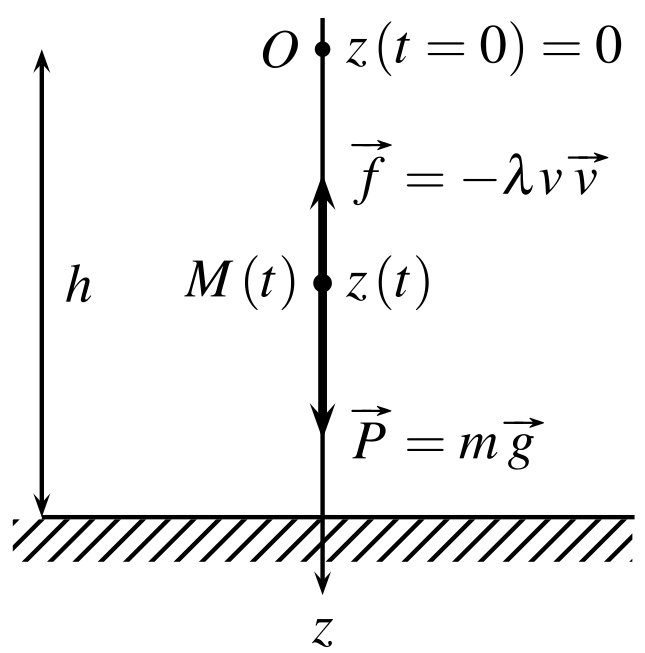
\includegraphics[width=\linewidth]{volant_corr}
		\end{center}
		\vspace{-30pt}
		\hfill~
	\end{minipage}\smallbreak
	\leftcenters{Ainsi,}{$\DS\boxed{\dv{v}{t} + \frac{\lb}{m}v^2 = g}$}
}

\QR{%
Montrer l'existence d'une vitesse limite $v_l$ et l'exprimer en
fonction de $\lambda$, $m$ et $g$.
}{%
Lorsqu'on lâche M sans vitesse initiale d'une hauteur $h$, la vitesse
est faible au départ et la force principale est le poids, accélérant le
mobile vers le bas. Quand la vitesse augmente, les frottements
s'intensifient jusqu'à ce qu'ils compensent le poids, donnant $\af =
	\of$~: la vitesse n'évolue plus et reste à sa valeur avant compensation,
la vitesse limite $v_l$. $v_l$ étant constante, $\vp_l = 0$, donc
l'équation différentielle donne
\[
	\frac{\lb}{m}v_l{}^2 = g
	\Lra
	\boxed{v_l = \sqrt{\frac{mg}{\lb}}}
\]
}

\enonce{%
	On note $t^* = t/\tau$, $z^* = z/L$ et $v^* = v/v_l$, avec $\tau = v_l/g$ et $L
		= v_l\tau$.
}

\QR{%
	Montrer que $t^*$, $z^*$ et $v^*$ sont trois grandeurs sans dimension.
}{%
	$v^*$ est le rapport de deux vitesses, donc est forcément sans
	dimension. Ensuite,
	\begin{gather*}
		[\tau] = \left[\frac{v_l}{g}\right] =
		\frac{\si{m.s^{-1}}}{\si{m.s^{-2}}} = \si{s}
		\\
		[L] = [v_l][\tau] = \si{m.s^{-1}}\times\si{s} = \si{m}
	\end{gather*}
	donc $\tau$ est bien un temps et $L$ une longueur~; ce faisant, $t^*$ et
	$z^*$ sont évidemment adimensionnées.
}

\QR{%
	Montrer que l'équation différentielle portant sur la vitesse peut se
	mettre sous la forme~:
	\[\dv{v^*}{t^*} + (v^*)^2 = 1\]
}{%
	On réécrit l'équation avec $v = v_lv^*$ et $t=\tau t^*$~:
	\begin{gather*}
		\dv{v}{t} + \frac{\lb}{m}v = g
		\Lra
		\dv{(v_lv^*)}{(\tau t^*)} + \frac{\lb}{m} \left(v_lv^*\right)^2 = g
		\Lra
		\frac{v_l}{\tau} \dv{v^*}{t^*} + \frac{\lb v_l{}^2}{m}(v^*)^2 = g
	\end{gather*}
	Or,
	\begin{gather*}
		\frac{v_l}{\tau} = g
		\qet
		\frac{\lb v_l{}^2}{m} = g
		\LRa
		\boxed{\dv{v^*}{t^*} + (v^*)^2 = 1}
	\end{gather*}
}
\enonce{%
	La résolution de l'équation précédente conduit à des solutions dont on donne les
	représentations graphiques ci-dessous.

	\begin{center}
		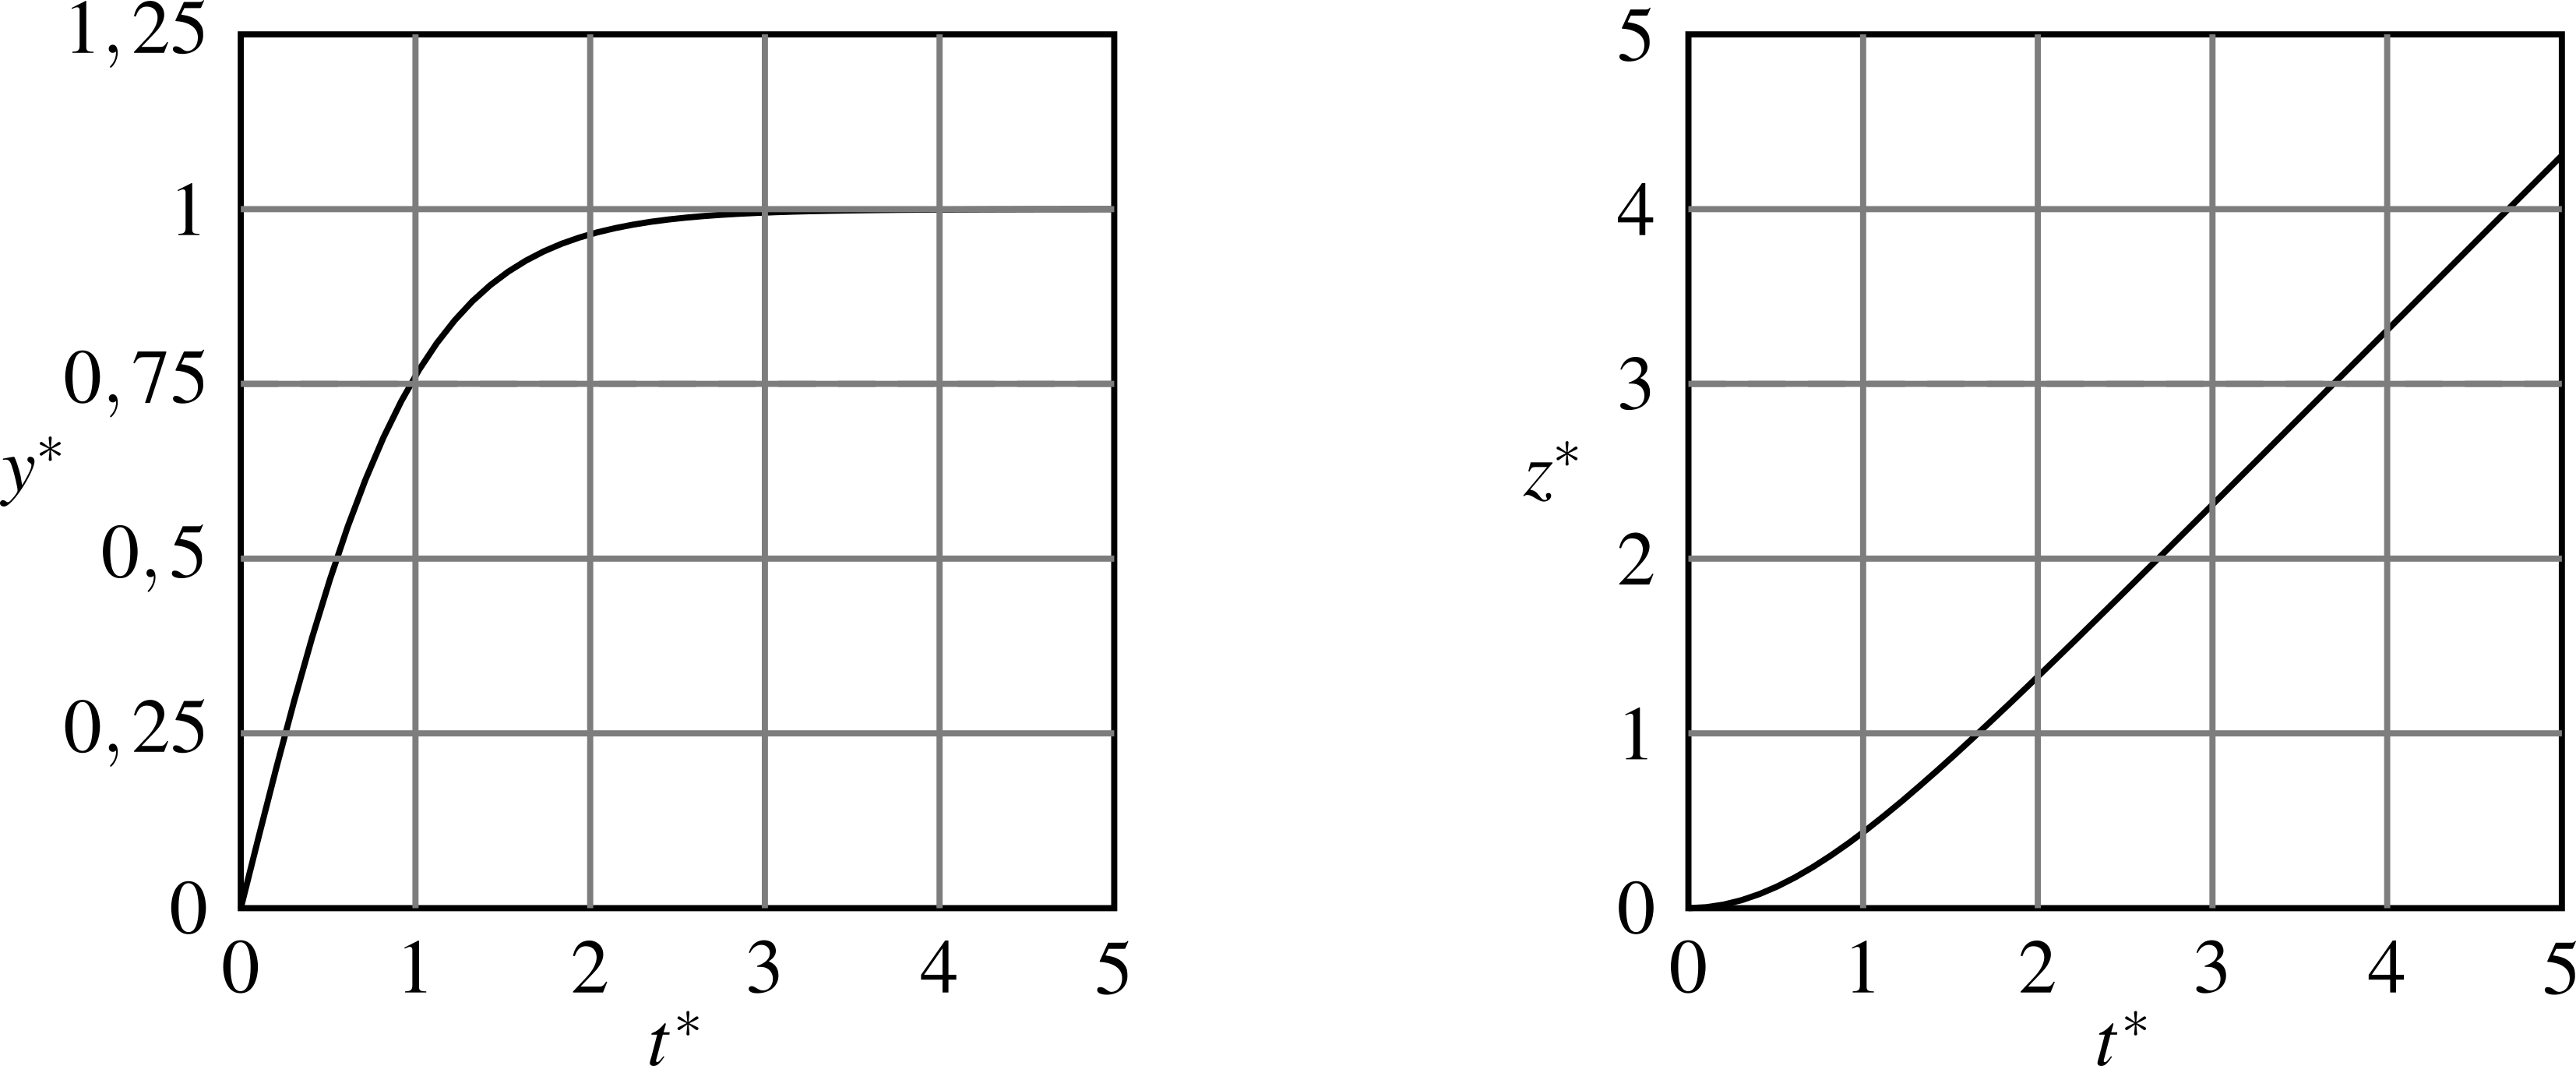
\includegraphics[width=.8\linewidth]{volant_data-plain}
	\end{center}
}

\QR{%
	À l'aide des courbes, décrire les deux phases du mouvement.
}{%
	Ces courbes montrent que la vitesse augmente pendant 2 à 3$\tau$,
	avant de se stabiliser à $v_l$. Le mouvement est ensuite rectiligne
	uniforme, et $z$ est une fonction affine du temps.
}
\QR{%
	Déterminer l'altitude minimale $h$ à laquelle il faut lâcher le volant
	pour que sa vitesse au sol soit supérieure ou égale à 95\% de $v_l$. On
	exprimera cette altitude en fonction de $L$. Déterminer également la
	durée $\D t$ de l'expérience en fonction de $\tau$.
}{%
	Le courbe représentant $v^*(t^*)$ montre que $v^* = \num{0.95}$ pour
	$t^* = \num{1.8}$. La durée de l'expérience pour arriver à cette valeur
	est donc $\SI{1.8}{\tau}$, et la hauteur $z^*$ à ce temps est $z^* =
		\num{1.2}$, ce qui correspond à $z = \SI{1.2}{L}$~; ainsi
	\[
		\boxed{\Dt = \SI{1.8}{\tau}}
		\qet
		\boxed{h = \SI{1.2}{L}}
	\]
}
\QR{%
	En admettant que la vitesse limite est proche de la valeur trouvée sur
	internet, calculer numériquement $L$ et $\tau$ puis $h$ et $\Dt$.
}{%
	En supposant $v_l$ connue, on a
	\begin{gather*}
		\tau = \frac{v_l}{g}
		\qet
		L = v_l\tau
		\qavec
		\left\{
		\begin{array}{rcl}
			v_l & = & \SI{25}{km.h^{-1}} = \SI{7.0}{m.s^{-1}} \\
			g   & = & \SI{9.81}{m.s^{-2}}
		\end{array}
		\right.\\
		\AN
		\boxed{\tau = \SI{7.1e-1}{s}}
		\qet
		\boxed{L = \SI{4.9}{m}}
	\end{gather*}
	Ainsi, \vspace*{-24pt}
	\begin{gather*}
		\Dt = \SI{1.8}{\tau}
		\qet
		h = \SI{1.2}{L}
		\\\Ra
		\boxed{\Dt = \SI{1.3}{s}}
		\qet
		\boxed{h = \SI{5.9}{m}}
	\end{gather*}
}
\end{document}
